The performance of LZW compression is influenced by the type of input data being processed. Different data types often exhibit varying compression ratios, as the efficiency of the algorithm depends on the frequency and patterns of repeating sequences within the input. For example, highly repetitive data tends to achieve better compression ratios, thereby reducing the computational workload per unit of compressed output. Conversely, inputs with little to no redundancy may lead to lower compression ratios and potentially increase the time required for dictionary operations. This relationship between data characteristics and compression efficiency underscores the need to evaluate LZW’s performance under diverse data scenarios.

\vspace{10pt}

% for English Text
When applied to English text, the complexity depends on the structure of the input. We will explore both the Best Case and Worst Case scenarios, supported by mathematical reasoning. Additionally, as the dictionary grows, operations like searching and updating may become more computationally expensive, which can further affect performance in scenarios with large or non-repetitive datasets.

\vspace{10pt}

\subsubsection{Best Case}
The best-case scenario for LZW compression occurs when the input data exhibit highly repetitive patterns, allowing the algorithm to use its dictionary efficiently. For example, an input like \textit{"aaaaaaa"} or \textit{"abababab"} is ideal. In this case:

\begin{itemize}
    \item After the initial iterations, most substrings encountered in the input are already present in the dictionary. The algorithm quickly matches these patterns with existing dictionary entries, minimizing the need for new insertions. Each search operation is $\mathcal{O}(1)$ on average when using a hash table for the dictionary.
    \item Since the input is repetitive, new entries are rarely added to the dictionary. As a result, the dictionary remains small, reducing memory usage and processing overhead. This efficient usage of the dictionary further enhances performance.
    \item The compression process involves scanning through the input and performing a constant-time dictionary lookup for each character. The overall complexity is $\mathcal{O}(L)$, where $L$ is the length of the input. The decompression process follows a similar pattern, as most patterns are reused, and the dictionary's small size ensures fast lookups. Thus, the complexity is $\mathcal{O}(L_c)$, where $L_c$ is the compressed data length.
\end{itemize}

\vspace{10pt}

The chart below displays the results of several test cases, each containing a string with repetitive patterns of varying lengths:

\begin{figure}[ht]
    \centering
    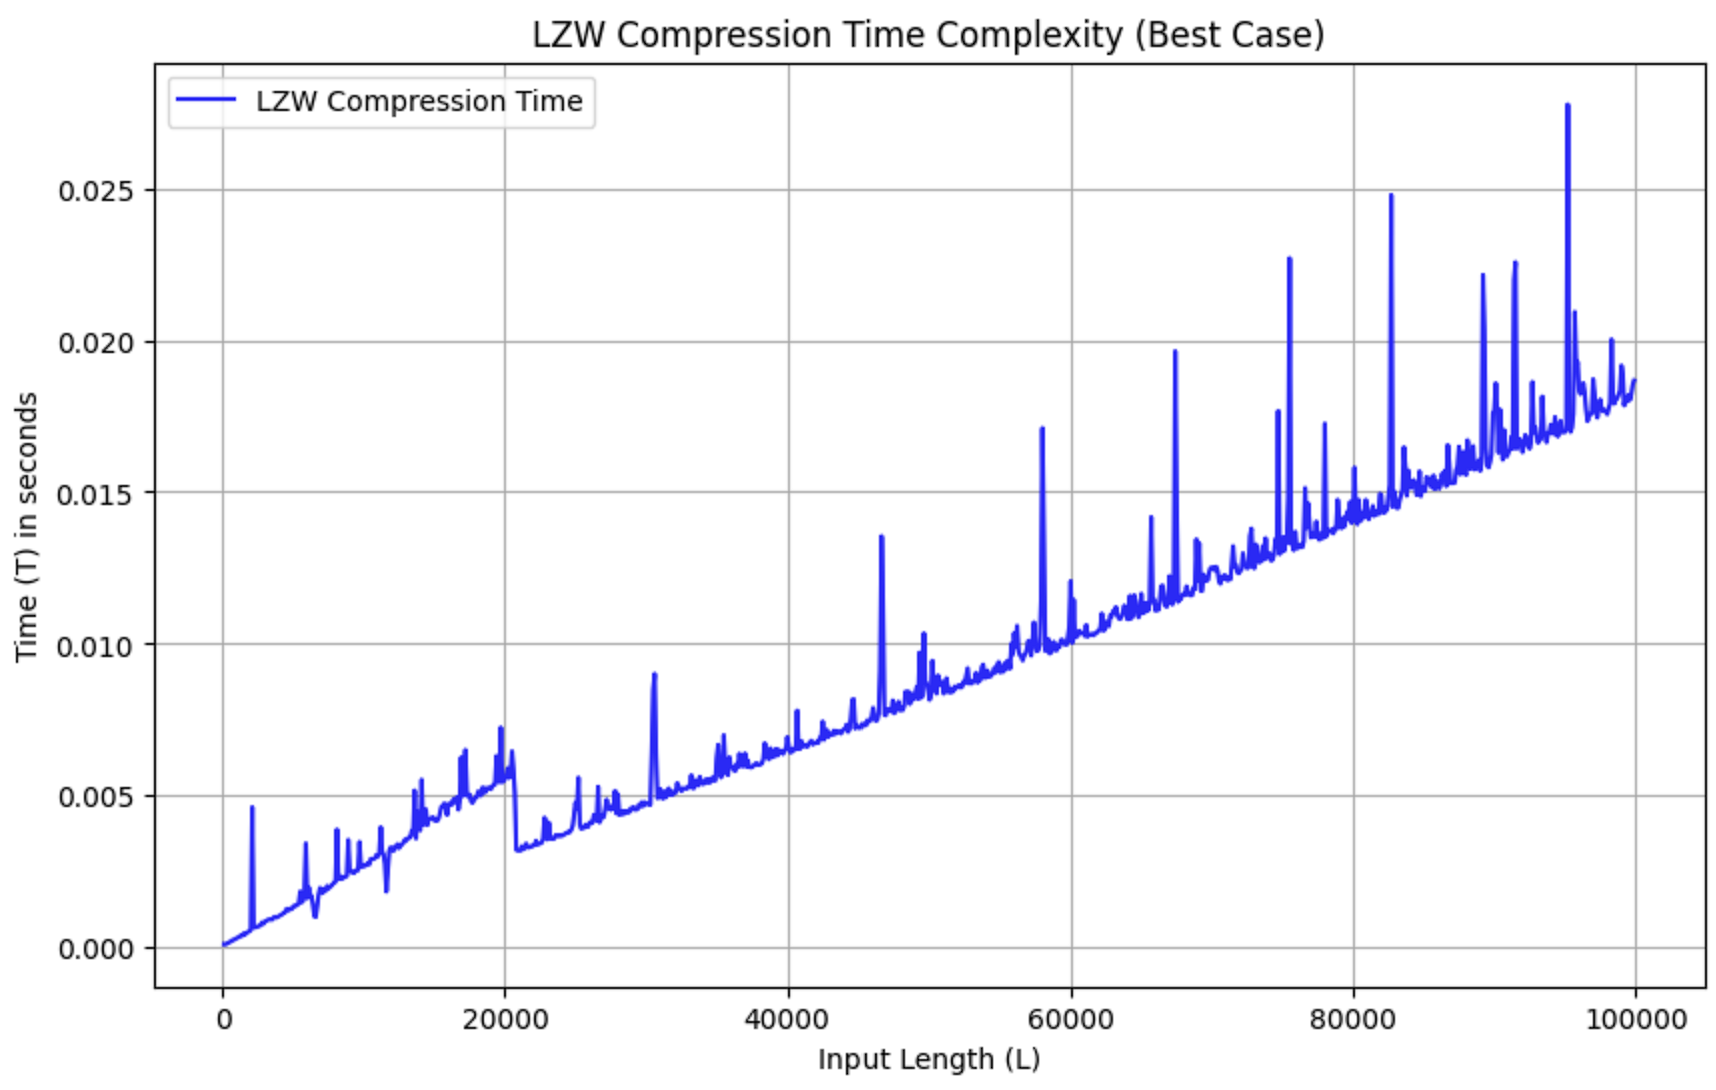
\includegraphics[width=0.8\linewidth]{Figures/best_case.png}
    \caption{LZW Compression Runtime in Best Case}
    \label{fig:bestcase}
\end{figure}

Based on this, we can prove that $T = \mathcal{O}(L)$ using the following chart:

\begin{figure}[ht]
    \centering
    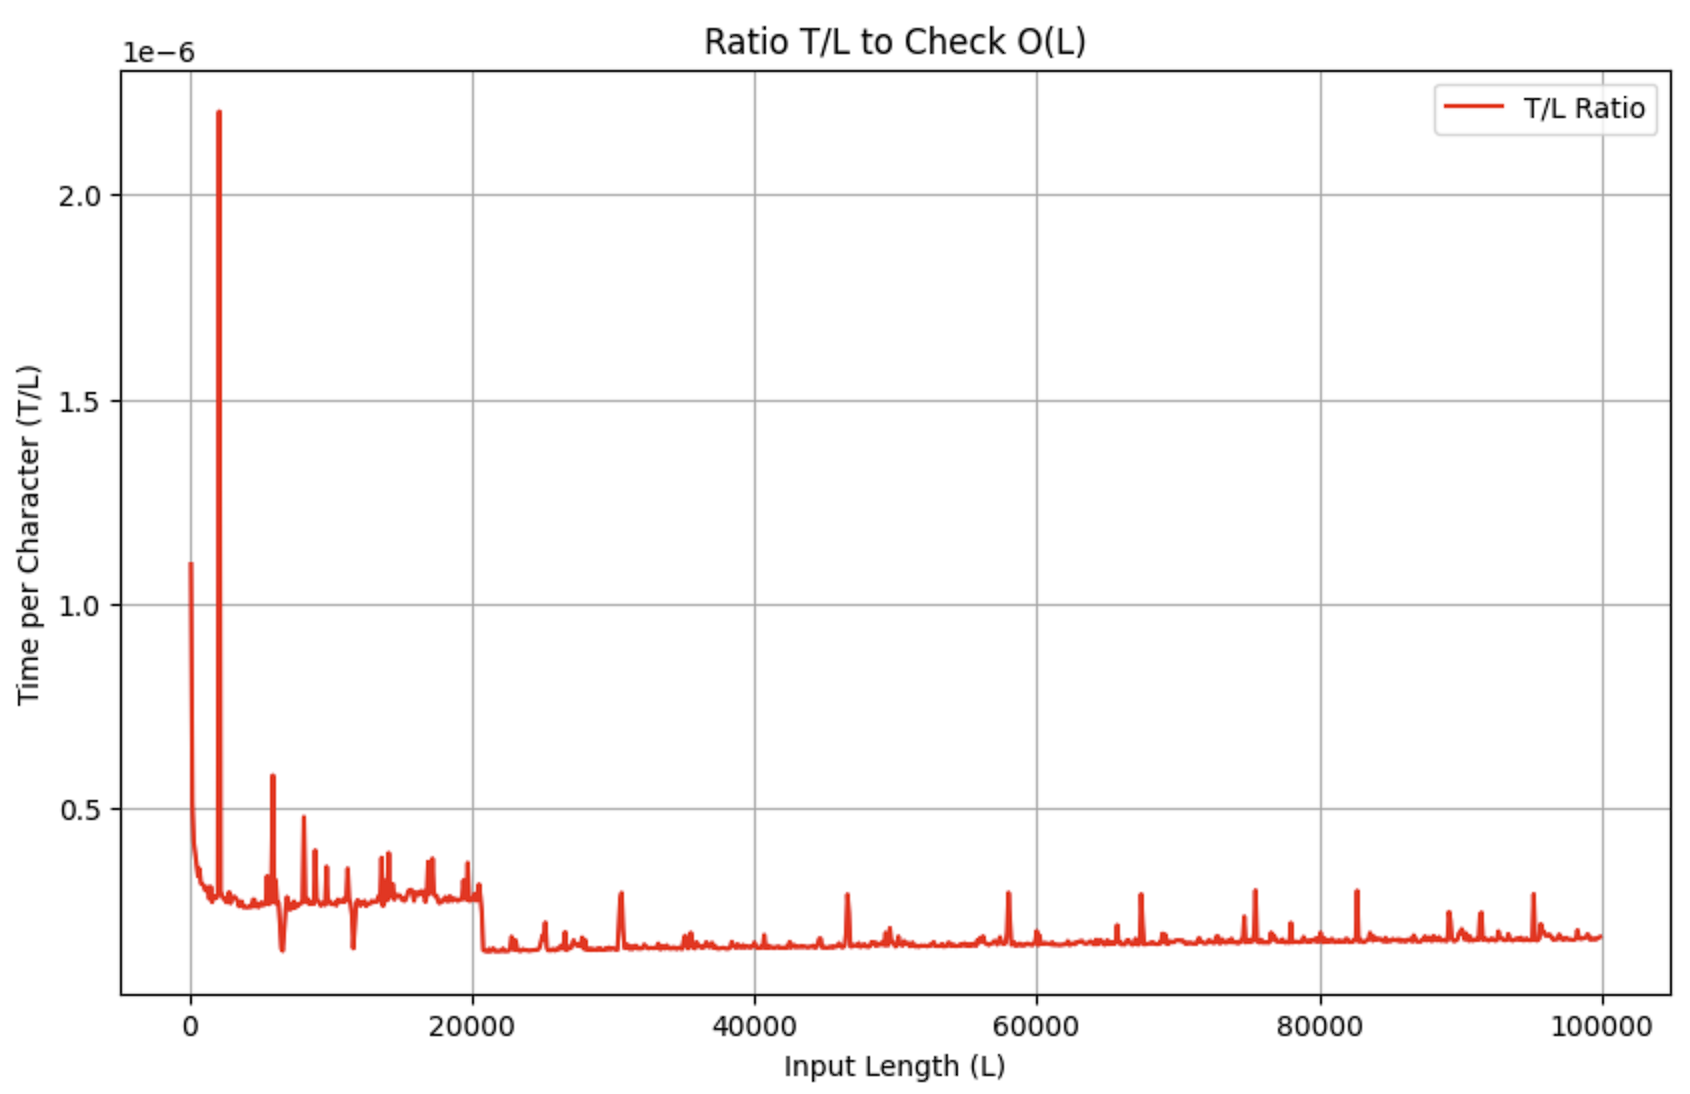
\includegraphics[width=0.8\linewidth]{Figures/bestcase_prove.png}
    \caption{Best Case: $T = \mathcal{O}(L)$}
    \label{fig:enter-label}
\end{figure}

\newpage

\subsubsection{Worst Case}
The worst-case scenario for LZW compression arises when the input data lacks any repetition or structure, such as unique or random characters. For example, an input like "abcdefg..." forces the algorithm to handle every substring as a new entity. In this case:

\begin{itemize}
    \item Every substring encountered in the input is unique and not found in the dictionary. This means that the algorithm frequently needs to perform dictionary insertions. Although lookups are $\mathcal{O}(1)$ on average, the frequent insertions can cause the dictionary size to grow rapidly.
    \item With each new substring, the dictionary expands, potentially reaching its maximum size $M$ quickly. If the dictionary size is not capped, this continuous growth consumes more memory and may degrade performance. In cases where a dictionary cap is implemented, frequent resets or replacements add additional overhead.
    \item Compression and decompression in the worst case are heavily affected by the rapid growth of the dictionary. Each character or code requires a dictionary lookup, and most substrings demand insertions. While the average-case lookup complexity remains $\mathcal{O}(1)$ with hash tables, poor hash distributions or collisions can degrade lookup performance to $\mathcal{O}(M)$, where $M$ is the dictionary size. Consequently, the compression complexity can reach $\mathcal{O}(L \cdot M)$, and the decompression complexity can grow to $\mathcal{O}(L_c \cdot M)$, where $L, L_c$ are the input and compressed lengths, respectively.
\end{itemize}

\vspace{10pt}

The following chart presents the results of multiple test cases, each containing a random string (barely repetitive) of different lengths:

\begin{figure}[ht]
    \centering
    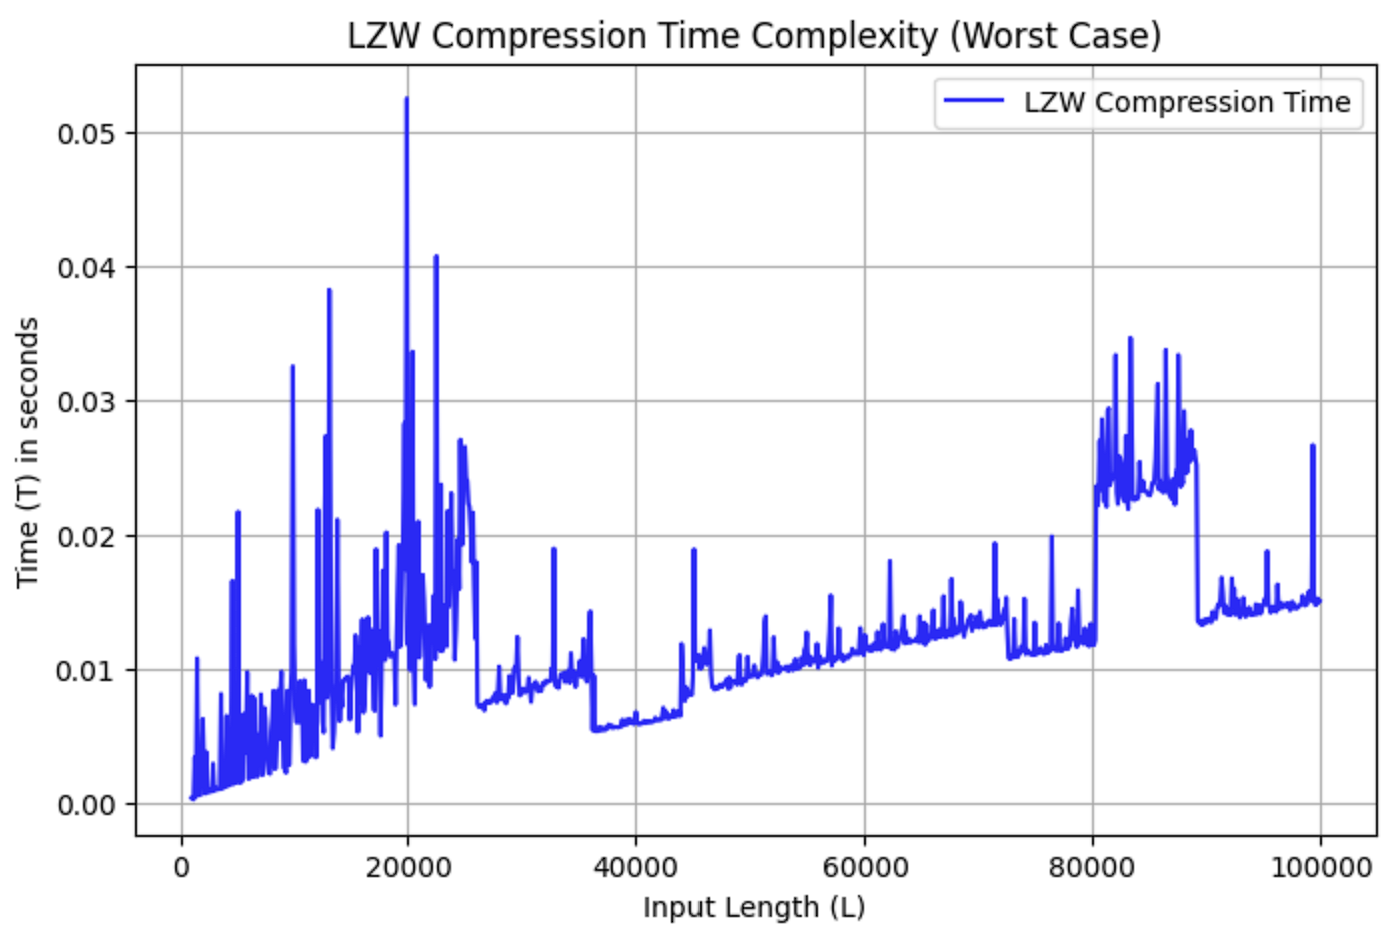
\includegraphics[width=0.8\linewidth]{Figures/worst_case.png}
    \caption{LZW Compression Runtime in Worst Case}
    \label{fig:worstcase}
\end{figure}

\newpage

From this, we can demonstrate that $T = \mathcal{O}(L \cdot M)$  through the following chart:

\begin{figure}[ht]
    \centering
    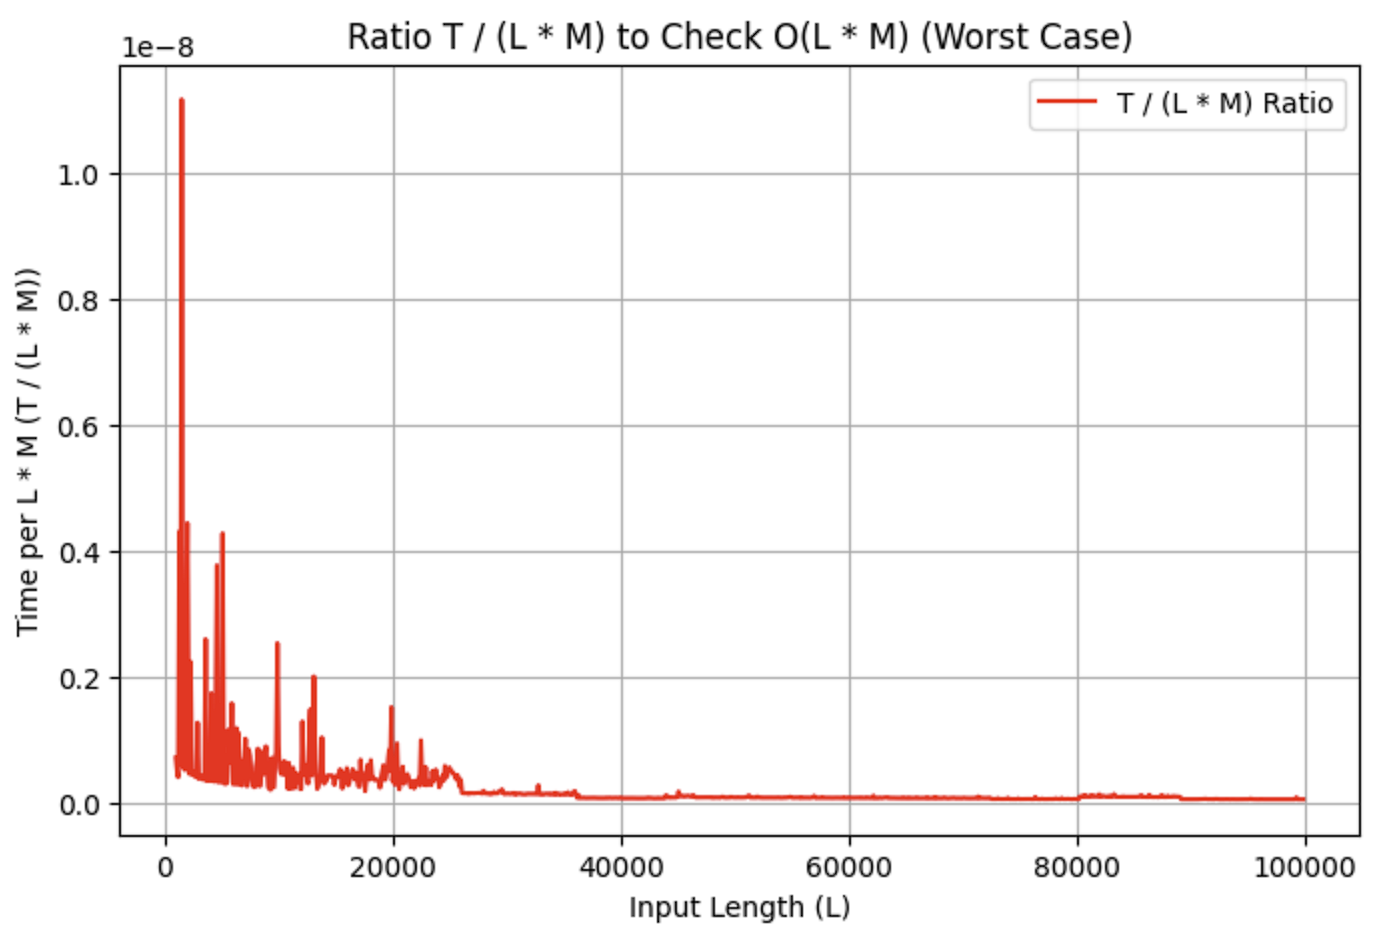
\includegraphics[width=0.8\linewidth]{Figures/worstcase_prove.png}
    \caption{Worst Case: $T = \mathcal{O}(L \cdot M)$}
    \label{fig:prove_worstcase}
\end{figure}